% /* GRASP: Copyright 1997,1998  Bruce Allen */
% $Id: man_frame.tex,v 1.37 1999/07/11 21:22:10 ballen Exp $
\section{GRASP Routines: Reading/using FRAME format data}
\setcounter{equation}0
\label{s:frameformat}
The LIGO and VIRGO projects have recently adopted a data format standard
called the FRAME format for time-domain data.  The 40-meter laboratory
at Caltech implemented this data format in Spring 1997; data taken after
that time is in the FRAME format.  The FRAME libraries are publicly
available from the VIRGO project; they may be downloaded from the site
\htmladdnormallink{{\tt http://wwwlapp.in2p3.fr/virgo/FrameL}.}
{http://wwwlapp.in2p3.fr/virgo/FrameL}
The GRASP package has been
tested up to release 3.72 of the frame library. Contact Benoit Mours\linebreak[4]
{\tt mours@lapp.in2p3.fr} for further information.

The GRASP package includes routines for reading and using data in the
FRAME format.  Also included in the GRASP package is a translator (see
Section~\ref{ss:translate}) which translates data from the old data format
used in 1994 to the new FRAME format.  Data distributed for use with
GRASP will primarily be distributed in this new FRAME format, and over
a period of time we will remove from the GRASP package all of the code
and routines which make use of the old format.  In order to help make
the transition from old format to FRAME format as smooth as possible,
the GRASP package currently contains both old format and FRAME format
versions of all of the example programs.  For example {\tt animate}
and {\tt animateF} are two versions of the same program.  The first
reads data in the old format, the second reads data in the FRAME format.
If you are new to GRASP, we don't recomend that you waste your time with
the old data format; start using the FRAME format immediately.

Data distributed in the FRAME format may not be compatible with future
releases of the FRAME library, so if the FRAME libraries are updated you
may need to obtain a new copy of the standard 40-meter test data set from
November 1994.  The data that has been distributed and is currently being
distributed makes use of either version 2.20, 2.30 or 2.37 of the
FRAME library.  We will shortly begin distributing data in version
3.50 of the FRAME format.
Only two files in the GRASP package ({\tt src/\-utility/\-frameinterface.c}
and {\tt src/\-examples/\-examples\_utility/\-translate.c}) depend upon the
version of the FRAME library.  We distribute GRASP with versions of
these files appropriate for different releases.
The files determine the version of the frame library at compilation
time, and then include the appropriate code.  This code works
correctly with any version of the frame library $2.37 \le {\rm
version} \le 3.70$.  Note that version $\ge 3.50$ of the frame library can
read data written by any version back to and including 2.37.

One of the nice properties of the FRAME formats $\ge 3.30$ is that
they support a ``compressed" format.  This is transparent to the user
(except that reading the ``compressed" frames takes a bit longer because the
frame library then needs to uncompress the data).  Data distributed in version
3.50 of the FRAME format is being distributed in this compressed form and
occupies somewhat less space than the old-format original data. As shown
in Section~\ref{s:40meter} the old-format data for the November 1994 runs
occupied about 13.6 Gbytes. For comparison, the FRAME-format data
occupies less than half of that space:
{\tt
\begin{verbatim}
     14nov94.1.frame 314
     14nov94.2.frame 397
     18nov94.1.frame 503
     18nov94.2.frame 543
     19nov94.1.frame 551   The space occupied
     19nov94.2.frame 535   is shown in Mbytes
     19nov94.3.frame 641
     19nov94.4.frame 605
     20nov94.1.frame 553
     20nov94.2.frame 422
     20nov94.3.frame 755
\end{verbatim}
}
\noindent
The total storage space required for FRAME 3.50 data totals only 5.8 Gbytes.

In order to give the 1994 40-meter data a form as similar as possible
to the data being taken in 1997 and beyond, the channel names used
have been given equivalent ``FRAME" forms.  These are shown in
Table~\ref{t:chassignf}.

Note that new data created in the frame format attempts to address at
least a couple of the problems in the ``old format" data.  In particular,
new frame format data (i.e., post 1996) has sample rate in Hz always being
powers of 2, for example, 4,096 Hz or 16 Hz or 16,384 Hz.  In addition,
each frame always contains a power-of-two number of seconds of data.
These conventions will make it easy to ``match up" sample of channels
taken at different rates, and to do FFT's of the channels.  However the
1994 data does not conform to either of these conventions: each frame of
1994 data contains 5000 samples of the slow channels, and 50,000 samples
of the fast channels, during a $5.06666\cdots$ second interval.

\begin{table}[h]
\begin{tabular}[]{c|c|c|c|c}
\hline
Channel \# & $\le$ 14 Nov 94 & FRAME name &  $\ge$ 18 Nov 94 & FRAME name\\
\hline
0 & IFO output & IFO\_DMRO & IFO output & IFO\_DMRO\\
1 & unused & & magnetometer & IFO\_Mag\_x \\
2 & unused &  & microphone & IFO\_Mike\\
3 & microphone & IFO\_Mike& unused & \\
\hline
4 & dc strain & IFO\_DCDM & dc strain & IFO\_DCDM \\
5 & mode cleaner pzt & PSL\_MC\_V & mode cleaner pzt & PSL\_MC\_V \\
6 & seismometer & IFO\_Seis\_1 & seismometer & IFO\_Seis\_1 \\
7 & unused & & slow pzt & IFO\_SPZT \\
8 & unused& & power stabilizer  & PSL\_PSS \\
9 & unused  & & unused & \\
10 & TTL locked & IFO\_Lock &  TTL locked & IFO\_Lock \\
11 & arm 1 visibility& IFO\_EAT & arm 1 visibility & IFO\_EAT\\
12 & arm 2 visibility & IFO\_SAT &  arm 2 visibility &  IFO\_SAT\\
13 & mode cleaner visibility & IFO\_MCR & mode cleaner visibility & IFO\_MCR\\
14 & slow pzt & IFO\_SPZT &  unused & \\
15 & arm 1 coil driver & SUS\_EE\_Coil\_V & arm 1 coil driver & SUS\_EE\_Coil\_V \\
\hline
\end{tabular}
Note: {\small On 18 November 1994 run 1 the power stabilizer was
accidentally disconnected until approximately 20:00 local time.}
\caption{Channel assignments for the November 1994 data runs.  Channels
0-3 are the ``fast" channels, sampled at about 10 kHz; the remaining
twelve are the ``slow" channels, sampled at about 1KHz.  The equivalent
``FRAME" format names are also given.}
\label{t:chassignf}
\end{table}
\clearpage

\subsection{Time-stamps in the November 1994 data-set}
\label{ss:timestamp}
\setcounter{equation}0
There is a serious problem in the original data format used in November
1994.  To understand the nature of this problem, remember that the
individual data samples (fast channels) are taken at about 10kHz,
so that the time between samples is about 100 $\mu$sec.  Ideally, the
time-stamps of the individual blocks should be recorded with a precision which
is substantially greater than this, i.e. a few $\mu$sec at the most.
However the November 1994 time stamps are recorded in two ways:  as an
integer number of seconds and msec (with 1000 $\mu$sec resolution) and
as a floating point elapsed time.  This latter quantity has a resolution
of less than one $\mu$sec at early times, but a resolution of about 2000
$\mu$sec at late times (say 15,000 sec into a run).

Thus, in translating the November 1994 data into frames (which have
1 nanosec resolution time-stamps), a reasonable effort was made
to ``correct" these time-stamps as much as possible, and to specify
the time at which each data block begins as precisely as possible.
After some research, we believe that the each block of old-format data is
precisely $76/15=5.0666666 \cdots$ seconds long.  So we have corrected
the time stamps accordingly.  One can show that in general, our time
stamps agree with those in the original data, when they are expressed
as floats, i.e. with the precison recorded in the original data set.
There are some blocks where there is an error in the least-significant
bit of the cast-into-float quantity; we do not understand this as well
as we would like.

Please, {\it be warned that the absolute time indicated by these stamps
is not correct!} These time stamps were not taken with a modern GPS clock
system, or even with an old-fashioned WWV system.  Our understanding is
that the real-time computer system on which these data were originally
taken had its clock set by wristwatch, with an accuracy of perhaps
$\pm 5$ minutes..  Indeed the computer system crashed on November 15,
1994 and the clock was subsequently reset again, so even the time
difference can not be trusted between November14 and November18 data.
It appears that the computer clock was not reset after November15th,
so the relative times in the remaining data may be trustworthy with
somewhat better than $\pm 1$ msec accuracy.

In any data anaysis work (such as pulsar searching) where it is
important to have precise time-stamps, these shortcomings must be taken
into account.  If you really want to determine the times more precisely
than a millisecond, our only suggestion is to examine the seismometer
data channel and correlate it with similar data taken by a system with
good time-stamps.  We don't know where to find such data, but it might
exist, somewhere, in the public domain.  If you do go to this trouble,
please write to us and tell us the conclusions of your study.  We would
be delighted to correct the absolute offset error in these November 1994
time-stamps, if someone could show us how to do it!
\clearpage

\subsection{Function: {\tt fget\_ch()} }
\setcounter{equation}0
{\tt int fget\_ch(struct fgetoutput *fgetoutput,struct fgetinput *fgetinput) }\\
\noindent
This is a general function for sequentially reading one or more
channels of FRAME format data.  It can be used to obtain either locked
sections only, or both locked and unlocked sections, and to retrieve
calibration information from the FRAME data.  It concatenates multiple
frames and multiple files containing frames as necessary, to return
continuous-in-time sequences.

The inputs to the routine {\tt fget\_ch()} are contained in a structure:
{\tt
\begin{verbatim}
struct fgetinput {
           int nchan;
           char **chnames;
           int npoint;
           short **locations;
           char *(*files)();
           int (*filedes)();
           int inlock;
           int seek;
           int calibrate;
           char *datatype; 
};
\end{verbatim}
}
The different elements of the structure are:
\begin{description}
\item{\tt nchan}: Input.  The number of channels that you want to retrieve ($ \ge 1$).
\item{\tt chnames}: Input.  The list of channel names.  Each element of
{\tt chnames[0..nchan-1]} is
   a pointer to a null-terminated string.  Note that the number of
   channels requested, and their names, must not be changed after the
   first call to {\tt fget\_ch}.  It is assumed that the first channel in
   the list has the fastest sample rate of any of the requested channels.
   As long as this assumption is satisfied, the channels may be accessed
   in any order.
\item{\tt npoint}: Input.  The number of points requested from the first channel.  (May change with each call.)
\item{\tt locations}: Input.  The locations in memory where the arrays corresponding to each channel should be placed
   are {\tt locations[0..nchan-1]}.   (May change with each call.)
\item{\tt files()}: Input.  A pointer to a function, which takes no
   arguments, and returns a pointer to a null-terminated character string.
   This string is the name of the file to look in for FRAME format data.
   If no further frames remain in the file, then the function {\tt
   files()} is called again.  When this function returns a null pointer,
   it is assumed that no further data remains.  A useful utility function
   called {\tt framefiles()} has been provided with GRASP, and may be
   used as this argument.  (May change with each call.)
\item{\tt filedes()}: Input.  This argument is used if and only if the
   previous argument, {\tt fgetinput.files} is {\tt NULL}.  If {\tt
   fgetinput.files} is not {\tt NULL} then this argument is not used.
   This argument is a pointer to a function, which takes no arguments,
   and returns an integer {\it file descriptor}.  The integer returned
   is a file descriptor for a file containing FRAME format data.  If no
   further frames remain in the file, then the function {\tt filedes()} is
   called again.  When this function returns a negative file descriptor,
   it is assumed that no further data remains.  (May change with each
   call.)
\item{\tt inlock}: Input.  Set to zero, return all data; set to non-zero, return only the locked sections of data.  If set nonzero, then on output {\tt fgetoutput.locklow} and {\tt fgetoutput.lockhi} will be set.
\item{\tt seek}: Input.  Set to zero, return data.  Set to non-zero,
   seek past the data, performing all normal operations, but do
   not actually write any data into the arrays pointed to by {\tt
   locations[0..nchan-1]}.  (May change with each call.)  This is useful
   for skipping rapidly past uninteresting regions of data, for example,
   the first few minutes after coming into lock.
\item{\tt calibrate}: Input.  If set non-zero, return calibration information.  If set to zero, do not return
   calibration information. (May change with each call.)
\item{\tt datatype}: Output. A character string indicating the data
   type in each channel. The coding is: C~= {\tt char}, S~= {\tt
     short}, D~= {\tt double}, F~= {\tt float}, I~= {\tt int}, L~= {\tt
     long}, f~= {\tt complex float}, d~= {\tt complex double}, s~= {\tt
     string}, u~= {\tt unsigned short}, i~= {\tt unsigned int}, l~=
     {\tt unsigned long}, c~= {\tt unsigned char}.  
\end{description}
\noindent
Except as noted above, it is assumed that none of these input arguments
are changed after the first call to {\tt fget\_ch()}.  It is also
assumed that within any given frame, the numbers of points contained
in different channels are exact integer multiples or fractions of the
numbers of points contained in the other channels.

The outputs from the routine {\tt fget\_ch()} are contained in a structure:
{\tt
\begin{verbatim}
struct fgetoutput {
           double tstart;
           double tstart_gps;
           double srate;
           int *npoint;
           int *ratios;
           int discarded;
           double tfirst;
           double tfirst_gps;
           double dt;
           double lostlock;
           double lostlock_gps;
           double lastlock;
           double lastlock_gps;
           int returnval;
           int frinum;
           float *fri;
           int tcalibrate;
           int tcalibrate_gps;
           int locklow;
           int lockhi;
           char *filename;
           char *slow_names; 
};
\end{verbatim}
}
The different elements of the structure are:
\begin{description}
\item{\tt  tstart}: Output. Time stamp of the first point output in channel {\tt chnames[0]}.
   Note: please see the comments in Section~\ref{ss:timestamp}.
Units are Unix-C time in seconds  defined in Section~\ref{s:timestandards}.
\item{\tt  tstart\_gps}: Output. Same as previous quantity, but with GPS time in seconds.
\item{\tt  srate}: Output.  Sample rate (in Hz) of channel {\tt chnames[0]}.
\item{\tt  npoint}: Output. The number of points returned in channel {\tt chnames[i]} is {\tt npoint[i]}.  Note
   that {\tt npoint[0]} is precisely the number of points requested in the input structure {\tt  fgetinput.npoint}.
\item{\tt  ratios}: Output.  The sample rate of channel {\tt chnames[0]} divided by the sample rate of
  channel {\tt chnames[i]} is given in {\tt ratios[i]}.  Thus {\tt ratios[0]=1}.
\item{\tt  discarded}: The number of points discarded from channel {\tt chnames[0]}.  These points are discarded
  because there is a missing period of time between two consecutive frames, or because the instrument was not in
  lock for long enough to return the requested number of points (or for both reasons).
\item{\tt  tfirst}: Output.  The time stamp of the first point returned in the first call to {\tt fget\_ch()}.   
Units are Unix-C time in seconds  defined in Section~\ref{s:timestandards}.
\item{\tt  tfirst\_gps}: Output.  Same as previous quantity, but with GPS time in seconds.
\item{\tt  dt}: Output.  By definition, {\tt tstart-tfirst}, which is the elapsed time since the first time stamp.
\item{\tt  lostlock}: Output.  The time at which we last lost lock (if searching only for locked segments).
Units are Unix-C time in seconds  defined in Section~\ref{s:timestandards}.
\item{\tt  lostlock\_gps}: Output.  Same as previous quantity, but with GPS time in seconds.
\item{\tt  lastlock}: Output.  The time at which we last regained lock (if searching only for locked segments).
Units are Unix-C time in seconds  defined in Section~\ref{s:timestandards}.
\item{\tt  lastlock\_gps}: Output.  Same as previous quantity, but with GPS time in seconds.
\item{\tt  returnval}: Output.  The return value of  {\tt fget\_ch()}:
  0 if it is unable to satisfy the request, 1 if the request has been
  satisfied by beginning a new locked or continuous-in-time section, and 2
  if the data returned is part of an ongoing locked or continuous-in-time
  sequence.
\item{\tt  frinum}: Output.  Three times the number of frequency values for which we are returning static calibration
    information.  If this number is not divisible by three, something is wrong!
\item{\tt  fri}: Output.  A pointer to the array of calibration data.  This data is arranged
 with a frequency, then the real part, then the imaginary part of
 the response, followed by another frequency, then real part, then
 imaginary part, etc.  So {\tt fri[0]=}$f_0$, {\tt fri[1]=}$r_0$,
 {\tt fri[2]=}$i_0$, {\tt fri[3]=}$f_1$, {\tt fri[4]=}$r_1$,
 {\tt fri[5]=}$i_1$,... and the total length of the array is {\tt
 fri[0..frinum-1]}.
\item{\tt  tcalibrate}: Output.  The time at which the current calibration information became valid.
Units are Unix-C time in seconds  defined in Section~\ref{s:timestandards}.
\item{\tt  tcalibrate\_gps}: Output.  Same as previous quantity, but with GPS time in seconds.
\item{\tt locklow}.  Output.  The minimum value (inclusive) for "in-lock" in the lock channel.
Set if and only if {\tt fgetinput.inlock} is nonzero.
\item{\tt lockhi}.  Output.  The maximum value (inclusive) for "in-lock" in the lock channel.
Set if and only if {\tt fgetinput.inlock} is nonzero.
\item{\tt filename}.  Output.  Points to a static character string containing
the name of the frame file currently in use, or {\tt NULL} is there is no
frame file open.
\item{\tt slow\_names}. Output. Names of the slow channels packed into one fast channel ``SLOW''.
\end{description}

Note that the time-stamps available in two different formats: Unix-C time in seconds 
and GPS time in seconds.  The relationship between these is described in detail in
Section~\ref{s:timestandards}.  In general, in new code the GPS time
stamps should be used, and taken as the more fundamental quantity.
The Unix-C time is the number of seconds after 00:00:00 Jan 1, 1970 UTC.
This is also known as
``Calendar Time" on Unix systems.  It is the quantity returned by the
Standard C-library function {\tt time()}.  Note that starting with
versions of the Frame library greater than 3.23, the time stored in the
frames is GPS time, which is (roughly - up to leap seconds) defined as the
Unix-C time minus $315964811$ (this value may be found
in the defined constant {\tt UTCTOGMT} in the {\tt grasp.h} header file.
The origin of GPS time is 00:00:00 January 6, 1980 UTC, which was
\begin{eqnarray*}
315964811 \ {\rm sec} &= & 3600 {\rm \ sec/hour} \times 24 {\rm \ hours/day} \times\\
& & (365 {\rm \ days/year} \times 8 {\rm \ years} + 366 {\rm \ days/year} \times 2 {\rm \ years}+ 5 {\rm \ days}) \\
& & + 11 {\rm\  leap\ sec}
\end{eqnarray*}
after 00:00:00 Jan 1, 1970 UTC.

This routine is a useful interface to the FRAME library.  It reads frames
from files.  To get the name of the first file to open, this routine
calls the function {\tt files()} specified in the input structure.
Then, whenever there are no remaining frames in this file, it calls {\tt
files()} again.  This function must return the name of the desired file,
or {\tt NULL} if no files remain.  For example:

\begin{verbatim}
static char *filelist[]={
"C1-94_11_19_23_50_46", "C1-94_11_19_23_53_28",
"C1-94_11_19_23_56_10", "C1-94_11_19_23_58_52",
"C1-94_11_20_00_01_34", "C1-94_11_20_00_04_16" };

char *files() {
     static int entry=0;
     if (entry>=6)
          return NULL;
     else
          return filelist[entry++];
}
\end{verbatim}
or the exact same fragment of code, but with:
\begin{verbatim}
static char *filelist[]={
"C1-468915467.F","C1-468915629.F","C1-468915791.F",
"C1-468915953.F","C1-468916115.F","C1-468916278.F" };
\end{verbatim}
The difference between the labeling of the frame files here is that
in the first instance (early versions of the frame library) the files
are assumed to be labeled by the UTC time in ``human-readable" form,
and in the latter case they are assumed to be labeled by the GPS time
in seconds.  Further details may be found in Section~\ref{ss:translate}
and Section~\ref{s:timestandards}.

The function {\tt fget\_ch()} returns 0 if it is unable to satisfy
the request for {\tt fgetinput.npoint} points.  It returns 1 if the
request has been satisfied, and it is beginning a new locked section
(or if the frames were not contiguous in time, and it is beginning with
a new frame).  It returns 2 if the data returned is part of an ongoing
locked or continuous sequence.

When several channels are requested, and they have different sample rates,
the first channel requested must always have the fastest sample rate.
Other requested channels may have this same sample rate, but none may
have a faster sample rate.  Points are returned from the slower channels
if and only if they satisfy the following condition.  Suppose that $r$
is the ratio of the channel 0 sample rate to the channel K sample rate,
and label the points in channel 0 by $i=0,\cdots,n r - 1$, and the
points in channel K by $j=0,\cdots,n-1$.  Then point $j$ in channel K
is returned if and only if point $i=rj$ is returned from channel 0.

\begin{description}
\item{Authors:}
Bruce Allen, ballen@dirac.phys.uwm.edu
\item{Comments:}
None.
\end{description}
\clearpage


\subsection{Function: {\tt framefiles()} }
\setcounter{equation}0
{\tt char *framefiles() }\\
\noindent
This is a ``utility function" for frame access.  It takes no arguments, and returns a pointer
to a static character string.  It is intended primarily as an argument to be passed to the
function {\tt fget\_ch()} via the structure member
{\tt fgetinput.files}.

The operation of the {\tt framefiles()} is determined by two environment
variables: {\tt GRASP\_FRAMEPATH}, and {\tt GRASP\_REALTIME}.  If {\tt
GRASP\_REALTIME} is set, then the {\tt framefiles()} interogates the EPICS
control system and returns a pointer to a character string containing the
name of the frame file most recently written to disk.  This option is
only intended for use in the 40-meter lab control room, for real-time
analysis of data.  For most users of GRASP, this option will never
be used.  Note: to set/unset the environment variable, use the commands:\\
\indent {\tt setenv GRASP\_REALTIME}\\
\indent {\tt unsetenv GRASP\_REALTIME}\\
respectively.

If the {\tt GRASP\_REALTIME} environment variable is NOT set, then the
behavior of {\tt framefiles()} is determined by the value of the {\tt GRASP\_FRAMEPATH}
environment variable.  This variable should point to a directory, and may be set with
a command like:\\
\indent {\tt setenv GRASP\_DATAPATH /usr/local/GRASP/data/18nov94.1frame}\\
The first time that {\tt framefiles()} is called, it looks for all
files with names of the type:\\
{\tt C1-*[0-9]}\\
{\tt C1-*.F}\\
{\tt H-*.F}\\
{\tt H-*.T}\\
{\tt L-*.F}\\
{\tt L-*.T}\\
in the directory pointed to by {\tt GRASP\_FRAMEPATH}.  These
correspond, respectively, to Caltech 40-m frame files labeled by date,
Caltech 40-m frame files labeled by GPS time, Hanford frame files,
Hanford trend frames, Livingston frame files, and Livingston trend
frames.  Note that the directory should contain files with only one
type of label:  if several label types exist in the directory, only the
files whose type matches the first entry found on the list above will
be used.   The labeling conventions are explained in
Section~\ref{ss:translate}.
The file names are stored internally, {\tt framefiles()} returns a pointer to 
a character string containing the name of the first of these files.  The
second call to {\tt framefiles()} returns the name of the second file found in the
directory, and so on.  When no more files remain, {\tt framefiles()} returns a NULL
pointer.

A simple way to analyze a subset of data is to create a directory
containing symbolic links to the FRAME files containing data that you want
to analyze, and to set the environment variable {\tt GRASP\_FRAMEPATH}
to point to that directory.

\begin{description}
\item{Authors:}
Bruce Allen, ballen@dirac.phys.uwm.edu
\item{Comments:}
None.
\end{description}
\clearpage



\subsection{Example: {\tt locklistF} program}
\setcounter{equation}0
This example uses the function {\tt fget\_ch} described in the
previous section to print out location information and times for all
the locked sections in the directory pointed to by the environment
variable {\tt GRASP\_FRAMEPATH}.
To run this program, type\\
\indent {\tt setenv GRASP\_FRAMEPATH /usr/local/GRASP/18nov94.1frame}\\
\indent {\tt locklistF}\\
and a list of locked time intervals will be printed out. 
Here is some typical output:
{\footnotesize \tt
\begin{verbatim}
locklistF
FrameL Version:April 10, 1997; v2.23(Apr 10 1997 18:32:52 ../src/FrameL.c)
GRASP: framefiles(): using 83 files from directory /ballen2/18nov94.1frame
Id: frameinterface.c,v 1.4 1997/04/30 07:00:39 ballen Exp 
Name: RELEASE_1_3  
In lock from t = 0.000000 into run to 526.450008 into run for 526.450008 sec
Out of lock from t = 526.450008 into run to 555.384692 into run for 28.934683 sec
In lock from t = 555.384692 into run to 667.775527 into run for 112.390835 sec
Out of lock from t = 667.775527 into run to 708.000798 into run for 40.225272 sec
In lock from t = 708.000798 into run to 2268.670924 into run for 1560.670125 sec
Out of lock from t = 2268.670924 into run to 2283.429062 into run for 14.758138 sec
In lock from t = 2283.429062 into run to 3954.517061 into run for 1671.088000 sec
Out of lock from t = 3954.517061 into run to 3966.367962 into run for 11.850901 sec
GRASP: fget_ch(): FRAMES NOT SEQUENTIAL
run 3 frame 842 ended at time: 785221840.948503 sec
run 3 frame 843 started at time: 785223012.765137 sec
Time gap is 1171.816634 sec
Gap starts 4266.133503 seconds into run; ends 5437.950137 seconds into run.
Discarding 294210 points remaining in the previous frame(s).
Id: frameinterface.c,v 1.4 1997/04/30 07:00:39 ballen Exp 
Name: RELEASE_1_3  
In lock from t = 3966.367962 into run to 4266.133503 into run for 299.765540 sec
Out of lock from t = 4266.133503 into run to 5437.950137 into run for 1171.816634 sec
GRASP: fget_ch(): FRAMES NOT SEQUENTIAL
run 3 frame 1040 ended at time: 785224015.965104 sec
run 3 frame 1041 started at time: 785224175.714844 sec
Time gap is 159.749740 sec
Gap starts 6441.150104 seconds into run; ends 6600.899844 seconds into run.
Discarding 132000 points remaining in the previous frame(s).
Id: frameinterface.c,v 1.4 1997/04/30 07:00:39 ballen Exp 
Name: RELEASE_1_3  
In lock from t = 5437.950137 into run to 6441.150104 into run for 1003.199968 sec
Out of lock from t = 6441.150104 into run to 6600.899844 into run for 159.749740 sec
In lock from t = 6600.899844 into run to 7375.472558 into run for 774.572714 sec
Out of lock from t = 7375.472558 into run to 7391.474039 into run for 16.001482 sec
In lock from t = 7391.474039 into run to 7685.337699 into run for 293.863659 sec
Out of lock from t = 7685.337699 into run to 7719.763049 into run for 34.425351 sec
In lock from t = 7719.763049 into run to 7973.647310 into run for 253.884261 sec
Out of lock from t = 7973.647310 into run to 8083.507974 into run for 109.860664 sec
In lock from t = 8083.507974 into run to 9160.715956 into run for 1077.207982 sec
Out of lock from t = 9160.715956 into run to 9220.780081 into run for 60.064125 sec
In lock from t = 9220.780081 into run to 10552.863624 into run for 1332.083544 sec
Out of lock from t = 10552.863624 into run to 10585.141461 into run for 32.277837 sec
In lock from t = 10585.141461 into run to 11466.650847 into run for 881.509386 sec
Out of lock from t = 11466.650847 into run to 11483.939559 into run for 17.288712 sec
In lock from t = 11483.939559 into run to 13268.796352 into run for 1784.856793 sec
Out of lock from t = 13268.796352 into run to 13297.379120 into run for 28.582768 sec
GRASP: fget_ch(): could not open NULL file name
had 0 points; still need 296000 points...
Discarding 0 points remaining in the previous frame(s).
Id: frameinterface.c,v 1.4 1997/04/30 07:00:39 ballen Exp 
Name: RELEASE_1_3  
\end{verbatim}
}

Note that this example only prints out information for locked sections
longer than 30 sec.  Also notice that because there are time gaps in
between some of the sucessive frames, error messages are printed out.
Notice the form of the GRASP error and warning messages.  These typically
begin with a line like:\\
{\tt 
\indent GRASP: fget\_ch(): this is the warning or error message\\ }
which specifies which GRASP function
the error messages come from.  They end with a pair of lines like\\ 
\indent {\tt Id: frameinterface.c,v 1.4 1997/04/30 07:00:39 ballen Exp \\
\indent Name: Name: RELEASE\_1\_3 \\ }
which are information about the file from which the warning or error message
came, including its version/release numbers.
Here is the code for the {\tt locklistF} example program:

\lgrindfile{Includes/locklistF.tex}
\clearpage

\subsection{Example: {\tt gwoutputF} program}
\setcounter{equation}0
This example uses the function {\tt fget\_ch()} described in the
previous section to print out a two-column file containing the IFO
output for the first locked section containing 100 sample points. 
To run this program, type\\
\indent {\tt setenv GRASP\_FRAMEPATH /usr/local/GRASP/18nov94.1frame}\\
\indent {\tt gwoutputF}\\
In the output, the left column is time values, and the right column
is the actual IFO output (note that because this comes from a 12 bit
A-D converter, the output is an integer value from -2047 to 2048).
The program works by acquiring data 100 points at a time, then printing
out the values, then acquiring 100 more points, and so on.  Whenever a
new locked section begins, the program prints a banner message to alert
the user.  Note that typical locked sections contain $\approx 10^7$
points of data, so this program should not be used for real work --
it's just a demonstration!
\lgrindfile{Includes/gwoutputF.tex}
\clearpage

\subsection{Example: {\tt animateF} program}
\label{s:animateF}
\setcounter{equation}0
This example uses the function {\tt fget\_ch()} described in the previous
section to produce an animated display showing the time series output
of the IFO in a lower window, and a simultaneously calculated FFT power
spectrum in the upper window. 
To run this program, type\\
\indent {\tt setenv GRASP\_FRAMEPATH /usr/local/GRASP/18nov94.1frame}\\
\indent {\tt animateF | xmgr -pipe}\\
This output from this program must be
piped into a public domain graphing program called {\tt xmgr}.  This may
be obtained from
\htmladdnormallink{{\tt http://plasma-gate.weizmann.ac.il/Xmgr/}.}
{http://plasma-gate.weizmann.ac.il/Xmgr/}
(This lists mirror sites in the USA and Europe also).
Some sample output of {\tt animateF} is shown in Figure~\ref{f:animateF}.
\begin{figure}[h]
\index{colorpage}
\begin{center}
\epsfig{file=Figures/figure7.ps,height=12cm,bbllx=15pt,bblly=60pt,
bburx=580pt,bbury=750pt}
\caption{ \label{f:animateF} Snapshot of output from {\tt animateF}.
This shows the (whitened) CIT 40-meter IFO a few seconds after acquiring
lock, before the violin modes have damped down }
\end{center}
\end{figure}

After compilation, to run the program type:\\
\indent {\tt animateF $|$ xmgr -pipe \&} \\
to get an animated display showing the data flowing by and the power
spectrum changing, starting from the first locked data.  You can also
use this program with command-line arguments, for example\\ \indent
{\tt  animateF 100 4 500 7 900 1.5 $|$ xmgr -pipe \&}\\ will show the
data from time $t= 100$ to time $t=104 $ seconds, then from $t=500$ to
$t=507$, then from $t=900$ to $t=901.5$.  Notice that the sequence of
start times must be increasing.  Note: the start times are measured relative
to the first data point in the first frame of data.

Note 1:  The {\tt xmgr} program as commonly distributed has a simple
bug that needs to be repaired, in order for the frequency scale of the
Fourier transform to be correct.  The corrected version of {\tt xmgr}
is shown in Figure~\ref{f:xmgrbugF}.
\begin{figure}
\hrulefill
{\tt
\begin{verbatim}
        case 0:
==>        delt=(x[ilen-1]-x[0])/(ilen-1.0);
==>        T=(x[ilen-1]-x[0]);
           setlength(cg,specset,ilen/2);
           xx=getx(cg,specset);
...

        case 1:
==>        delt=(x[ilen-1]-x[0])/(ilen-1.0);
==>        T=(x[ilen-1]-x[0]);
\end{verbatim}}
\caption{\label{f:xmgrbugF} The corrections to a bug in the {\tt xmgr}
program are indicated by the arrows above.  This bug is in the routine
{\tt do\_fourier()} in the file {\tt computils.c}. This bug has been
corrected in {\tt xmgr} version 4.1 and greater.}
\hrulefill
\end{figure}


Note 2: Two closely related programs {\tt animateT} and {\tt
    animateF}
are also included.  {\tt animateT} is identical to {\tt animateF}
except that it does {\it not} assume that the data is in shorts.
Hence it is appropriate, for example, for producing an animated
display of `trend' files in which frames contain channels stored as doubles.
{\tt animateS} is designed to produce an animated 
display of  data from a channel name `SLOW'.
This channel is used as a way of packing a approximately 230 channels sampled
at 1Hz into a single fake channel (incorrectly labelled with sample
rate 256Hz). 


\lgrindfile{Includes/animateF.tex}


 

\clearpage

\subsection{Swept-sine calibration information}
\setcounter{equation}0

The swept sine calibration files are 3-column ASCII files, of the form:
\begin{center}
$f_0$ $\qquad$ $r_0$ $\qquad$ $i_0$ \\
$f_1$ $\qquad$ $r_1$ $\qquad$ $i_1$ \\
$f_2$ $\qquad$ $r_2$ $\qquad$ $i_2$ \\
$\cdots$\\
$f_m$ $\qquad$ $r_m$ $\qquad$ $i_m$
\end{center}
where the $f_j$ are frequencies, in Hz, and $r_j$ and $i_j$ are
dimensionless ratios of voltages. 
There are typically $m=801$ lines in
these files.  
The data from these files (as well as one additional line of the
form\\
0.0  0.0  0.0\\
showing vanishing response at DC) have been included in the frames.
Each line gives the ratio of the IFO output voltage to a
calibration coil driving voltage, at a different frequency.  The $r_j$
are the ``real part" of the response, i.e. the ratio of the IFO output
in phase with the coil driving voltage, to the coil driving voltage.
The $i_j$ are the ``imaginary part" of the response, $90$ degrees out
of phase with the coil driving voltage.  The sign of the phase (or
equivalently, the sign of the imaginary part of the response) is
determined by the following convention.  Suppose that the driving
voltage (in volts) is
\begin{equation}
\label{e:calibrate1F}
V_{\rm coil} = 10 \cos( \omega t) = 10 \Re {\rm e}^{i \omega t}
\end{equation}
where $\omega= 2 \pi \times 60 \> {\rm radians/sec}$ is the angular frequency of
a 60 Hz signal.  Suppose the
response of the interferometer output to this is (again, in volts)
\begin{eqnarray}
\label{e:calibrate2F}
V_{\rm IFO} &=& 6.93 \; \cos(\omega t) + 4\; \sin(\omega t)\cr
 &=& 6.93 \; \cos(\omega t) - 4\; \cos(\omega t + \pi/2) \cr
 &=& 8 \; \Re {\rm e}^{i (\omega t - \pi/6)}
\end{eqnarray}
This is shown in Figure~\ref{f:phaseF}. 
An electrical engineer would describe this
situation by saying that the phase of the response $V_{\rm IFO}$ is lagging the
phase of the driving signal $V_{\rm coil}$ by $30^\circ$.  The corresponding line
in the swept sine calibration file would read:
\begin{center}
$\cdots$\\
$60.000$ $\qquad$ $0.6930$ $\qquad$ $-0.40000$\\
$\cdots$
\end{center}
Hence, in this example, the real part is positive and the imaginary
part is negative.  We will denote this entry in the swept sine
calibration file by $S(60) = 0.8 \; {\rm e}^{ -i\pi/6} = 0.693 - 0.400
i$.  Because the interferometer output is real, there is also a value
implied at negative frequencies which is the complex conjugate of the
positive frequency value:  $S(-60) = S^*(60) = 0.8 \; {\rm e}^{
i\pi/6} = 0.693 + 0.400 i$.

Because the interferometer has no DC response, it is convenient for us
to add one additional point at frequency $f=0$ into the output data
arrays, with both the real and imaginary parts of the response set to
zero.  Hence the output arrays contain one element more than the number
of lines in the input files.  Note that both of these arrays are
arranged in order of increasing frequency; after adding our one
additional point they typically contain 802 points at frequencies from
0 Hz to 5001 Hz.

For the data runs of interest in this section (from
November 1994) typically a swept sine calibration curve was taken
immediately before each data tape was generated.

\begin{figure}[t]
\begin{center}
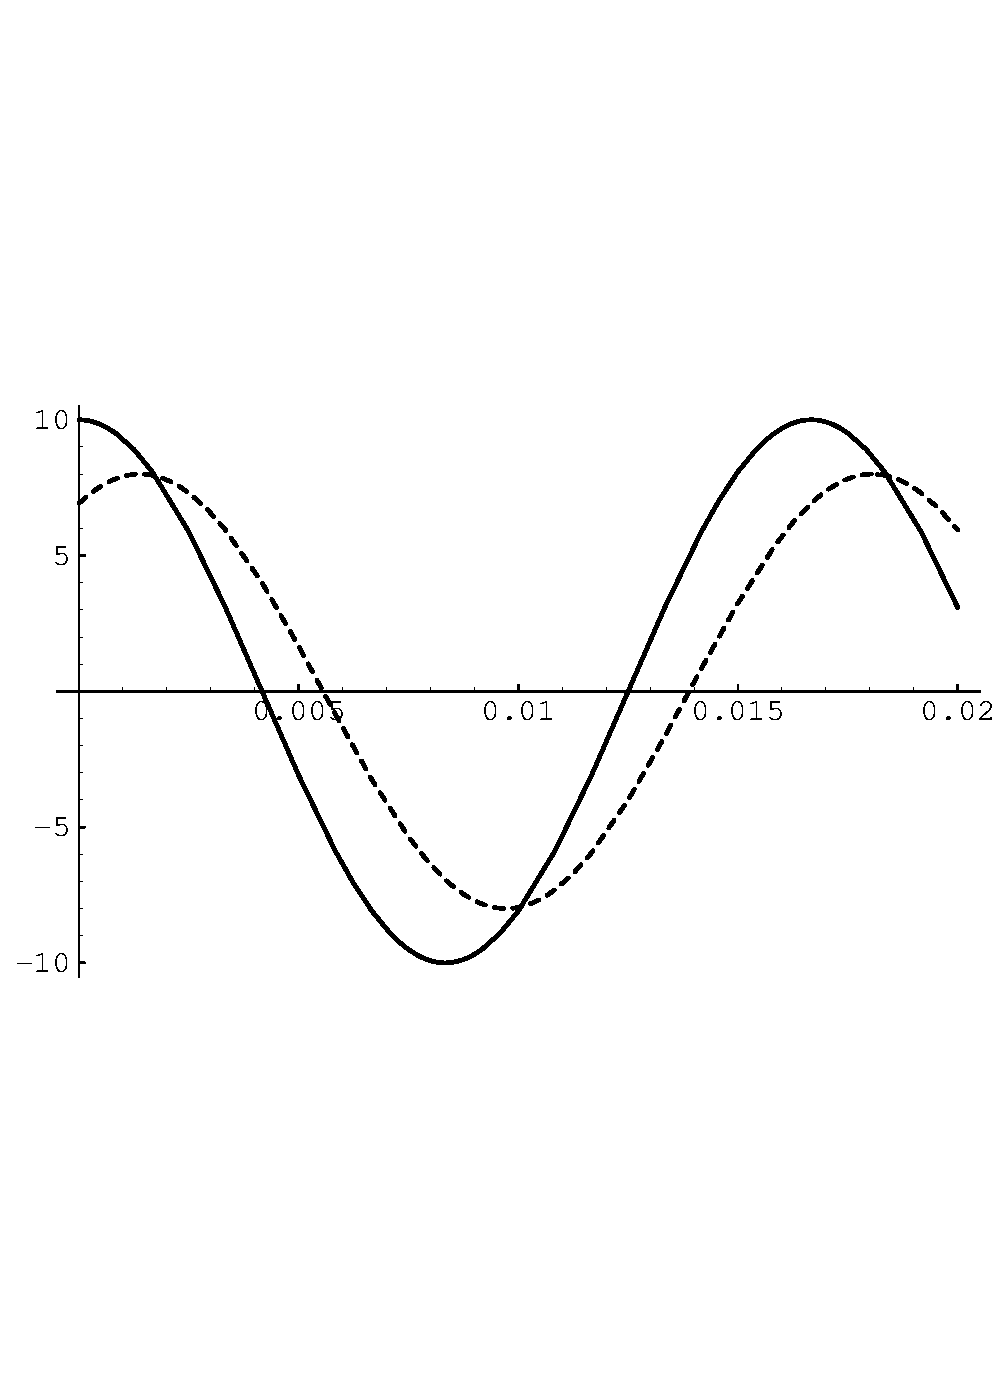
\epsfig{file=Figures/figure8.ps,height=5cm,bbllx=60pt,bblly=250pt,
bburx=550pt,bbury=530pt}
\caption{ \label{f:phaseF} This shows a driving voltage $V_{\rm coil}$
(solid curve) and the response voltage $V_{\rm IFO}$ (dotted curve) as
functions of time (in sec).  Both are 60 Hz sinusoids; the relative
amplitude and phase of the in-phase and out-of-phase components of
$V_{\rm IFO}$ are contained in the swept-sine calibration files.}
\end{center}
\end{figure}

We will shortly address the following question.  How does one use the
dimensionless data in the swept-sine calibration curve to reconstruct the
differential motion $\Delta l(t)$ (in meters) of the interferometer
arms?  Here we address the closely related question:  given $V_{\rm
IFO}$, how do we reconstruct $V_{\rm coil}$?  We choose the sign
convention for the Fourier transform which agrees with that of {\it
Numerical Recipes}:  equation (12.1.6) of \cite{NumRec}.  The Fourier
transform of a function of time $V(t)$ is
\begin{equation}
\label{e:fft1F}
{\tilde V}(f) = \int {\rm e}^{2 \pi i f t} V(t) dt.
\end{equation}
The inverse Fourier transform is
\begin{equation}
\label{e:fft2F}
V(t)= \int {\rm e}^{-2 \pi i f t} {\tilde V}(f) df.
\end{equation}
With these conventions, the signals (\ref{e:calibrate1F}) and
(\ref{e:calibrate2F}) shown in in Figure~\ref{f:phaseF} have Fourier
components:
\begin{eqnarray}
{\tilde V}_{\rm coil}(60) = 5                  \quad &{\rm and}& \quad {\tilde V}_{\rm coil}(-60) = 5,\\
{\tilde V}_{\rm IFO}(60)  = 4{\rm e}^{i \pi/6} \quad &{\rm and}& \quad {\tilde V}_{\rm IFO}(-60)  = 4 {\rm e}^{-i \pi/6}.
\end{eqnarray}
At frequency $f_0=60$ Hz the swept sine file
contains
\begin{equation}
S(60) = 0.8 \; {\rm e}^{-i \pi/6} \Rightarrow S(-60) = S^*(60) =
0.8 \; {\rm e}^{i \pi/6}.
\end{equation}
since $S(-f) = S^*(f)$.

With these choices for our conventions, one can see immediately from our
example (and generalize to all frequencies) that
\begin{equation}
\label{e:coilconF}
{\tilde V}_{\rm coil}(f) = {{\tilde V}_{\rm IFO} \over S^*(f)}.
\end{equation}
In other words, with the {\it Numerical Recipes} \cite{NumRec}
conventions for forward and reverse Fourier Transforms, the (FFT of
the) calibration-coil voltage is  the (FFT of the) IFO-output
voltage divided by the complex conjugate of the swept sine response.
\begin{description}
\item{Author:}  Bruce Allen, ballen@dirac.phys.uwm.edu
\item{Comments:}  The swept-sine calibration curves are usually quite
smooth but sometimes they contain a ``glitch" in the vicinity of
1 kHz; this may be due to drift of the unity-gain servo point.
\end{description}
\clearpage

\subsection{Function: {\tt GRcalibrate()}}
\label{ss:GRcalibrate}
\setcounter{equation}0
{\tt void GRcalibrate(float *fri,int frinum,int num,float *complex,float srate,int method,int order) }\\
This is a intermediate-level routine which 
takes as input a pointer to an array containing the swept sine data, and
outputs an array of interpolated points suitable for calibration of
FFT's of the interferometer output.

The arguments are:
\begin{description}
\item{\tt fri:} Input.  Pointer to an array containing
  swept sine data.  The format of this data is {\tt fri[0]=}$f_0$,
{\tt fri[1]=}$r_0$, {\tt fri[2]=}$i_0$,
{\tt fri[3]=}$f_1$,
{\tt fri[4]=}$r_1$, {\tt fri[5]=}$i_1$,... and the total length of the
array is {\tt fri[0..frinum-1]}.
\item{\tt frinum:} Input.  The number of entries in the array  {\tt fri[0..frinum-1]}.
If this number is not divisible by three, something is wrong!
\item{\tt num:} Input.  The number of points $N$ in the FFT that we
 will be calibrating.  This is typically $N=2^k$ where $k$ is an
 integer.  In this case, the number of distinct frequency values at
 which a calibration is needed is $2^{k-1}+1 = N/2+1$, corresponding to
 the number of distinct frequency values from $0$ (DC) to the Nyquist
 frequency $f_{\rm Nyquist}$.  See for example equation (12.1.5) of
 reference \cite{NumRec}.  The frequencies are $f_i = {i \over N}
 F_{\rm sample}$ for $i=0,\cdots,N/2$.
\item{\tt srate:} Input.  The sample rate $F_{\rm sample}$ (in Hz) of the data that
  we are going to be calibrating.
\item{\tt complex:} Input.  Pointer to an array {\tt complex[0..s]}
  where $s=2^k+1$.  The routine {\tt  calibrate()} fills in this array
  with interpolated values of the swept sine calibration data,
  described in the previous section.  The real part of the DC response
  is in {\tt complex[0]}, and the imaginary part is in {\tt
  complex[1]}. The real/imaginary parts of the response at frequency
  $f_1$ are in {\tt complex[2]} and {\tt complex[3]} and so on.  The
  last two elements of {\tt complex[ ]} contain the real/imaginary parts
  of the response at the Nyquist frequency $F_{\rm sample}/2$.
\item{\tt method:} Input.  This integer sets the type of interpolation
  used to determine the real and imaginary part of the response, at
  frequencies that lie in between those given in the swept sine
  calibration files.  Rational function interpolation is used if {\tt
  method}=0.  Polynomial interpolation is used if {\tt method}=1.
  Spline interpolation with natural boundary conditions (vanishing
  second derivatives at DC and the Nyquist frequency) is used if {\tt
  method}=2.
\item{\tt order:}  Input.  Ignored if spline interpolation is used.
  If polynomial interpolation is used, then {\tt order} is the order
  of the interpolating polynomial.
  If rational function interpolation is used, then the numerator and
  denominator are both polynomials of order {\tt order}/2 if {\tt order}
  is even; otherwise the degree of the denominator is ({\tt order}+1)/2
  and that of the numerator is ({\tt order}-1)/2.
\end{description}

The basic problem solved by this routine is that the swept sine
calibration data in a frame typically contain data at a few hundred
distinct frequency values.   However to properly calibrate the IFO output,
one usually needs this calibration information at a large number of
frequencies corresponding to the distinct frequencies associated with the
FFT of a data set.  This routine allows you to choose different possible
interpolation methods.  If in doubt, we recommend spline interpolation
as the first choice.  The interpolation methods are described in detail
in Chapter 3 of reference \cite{NumRec}.
\begin{description}
\item{Author:}  Bruce Allen, ballen@dirac.phys.uwm.edu
\item{Comments:}  It might be better to interpolate values of
$f^2$ times the swept-sine response function, as this is the quantity
needed to compute the IFO response function.
\end{description}
\clearpage

\subsection{Example: {\tt print\_ssF} program}
\label{ss:print_ssF}
\setcounter{equation}0
This example uses the function {\tt GRcalibrate()} to read the swept
sine calibration information from a frame, and then prints out a list
of frequencies, real, and imaginary parts interpolated from this data.
The frequencies are appropriate for the FFT of a 4096 point data set with
sample rate {\tt srate}.   The technique used is spline interpolation.
To run this program, and display a graph, type\\
\indent {\tt setenv GRASP\_FRAMEPATH /usr/local/GRASP/18nov94.1frame}\\
\indent {\tt print\_ssF > outputfile}\\
\indent {\tt xmgr -nxy outputfile}\\

\lgrindfile{Includes/print_ssF.tex}

\begin{figure}[h]
\begin{center}
\epsfig{file=Figures/swept.ps,angle=-90,bbllx=40pt,bblly=72pt,
bburx=580pt,bbury=720pt,width=5.0in}
\index{colorpage}
\caption{ \label{f:swept}
A swept sine calibration curve, showing the real and imaginary parts, produced by
the example program {\tt print\_ssF}.}
\end{center}
\end{figure}

\clearpage
\subsection{Function: {\tt GRnormalize()}}
\label{s:normalizeF}
\setcounter{equation}0
{\tt void GRnormalize(float *fri, int frinum, int npoint, float srate,float *response)}

This routine generates an array of complex numbers $R(f)$ from
the swept sine information in a frame, and an overall calibration
constant.  Multiplying this array of complex numbers by (the FFT of)
the raw IFO data yields the (FFT of the) differential displacement of
the interferometer arms $\Delta l$, in meters: $\widetilde{\Delta l}(f)
= R(f) \widetilde{C_{\rm IFO}}(f)$.  The units of $R(f)$ are meters/ADC-count.

The arguments are:
\begin{description}
\item{\tt fri:} Input.  Pointer to an array containing
  swept sine data.  The format of this data is {\tt fri[0]=}$f_0$,
{\tt fri[1]=}$r_0$, {\tt fri[2]=}$i_0$,
{\tt fri[3]=}$f_1$,
{\tt fri[4]=}$r_1$, {\tt fri[5]=}$i_1$,... and the total length of the
array is {\tt fri[0..frinum-1]}.
\item{\tt frinum:} Input.  The number of entries in the array  {\tt fri[0..frinum-1]}.
If this number is not divisible by three, something is wrong!
\item{\tt npoint:} Input.  The number of points $N$ of IFO output which will be used
to calculate an FFT for normalization.
Must be an integer power of 2.
\item{\tt srate:}  Input.  The sample rate in Hz of the IFO output.
\item{\tt response:} Output.  Pointer to an array {\tt response[0..s]}
with $s=N+1$ in which $R(f)$ will be returned.   By convention,
$R(0)=0$ so that {\tt response[0]=response[1]=0}.    Array elements
{\tt response[$2 i$]} and {\tt response[$2 i + 1$]} contain the real and
imaginary parts of $R(f)$ at frequency $f= i{\tt srate}/N$.   The
response at the Nyquist frequency {\tt response[N]=0} and {\tt
response[N+1]=0} by convention.
\end{description}

The absolute normalization of the interferometer can be obtained from
the information in the swept sine file, and one other normalization
constant which we denote by $Q$.  It is easy to understand how this
works.  In the calibration process, one of the interferometer end
mirrors of mass $m$ is driven by a magnetic coil.  The equation of
motion of the driven end mass is
\begin{equation}
m {d^2 \over dt^2} {\Delta l} = F(t)
\end{equation}
where $F(t)$ is the driving force and $\Delta l$ is the differential
length of the two interferometer arms, in meters.  Since the driving
force $d(t)$ is proportional to the coil current and thus to the coil
voltage, in frequency space this equation becomes
\begin{equation}
(- 2 \pi i f)^2 \widetilde{\Delta l}  = {\rm constant} \times \widetilde{V}_{\rm coil} =
{\rm constant} \times {{\tilde V}_{\rm IFO} \over S^*(f)}.
\end{equation}
We have substituted in equation (\ref{e:coilconF}) which relates
${\tilde V}_{\rm IFO}$ and ${\tilde V}_{\rm coil}$.
The IFO voltage is directly proportional to the quantity recorded in 
the IFO output channel: $V_{\rm IFO} = {\rm ADC} \times C_{\rm IFO}$, with the constant ${\rm ADC}$ 
being the ratio of the analog-to-digital converters input voltage to
output count.

Putting together these factors, the
properly normalized value of $\Delta l$, in meters, may be obtained
from the information in the IFO output channel, the swept sine calibration information, and the
quantities given in Table~\ref{t:unitsF} by
\begin{equation}
\label{e:rdefF}
\widetilde{\Delta  l} = R(f) \times \widetilde{C_{\rm IFO} }  \qquad {\rm with } \quad
R(f) = {Q  \times {\rm ADC}  \over -4 \pi^2 f^2 S^*(f)},
\end{equation}
where the $\tilde {}$ denotes Fourier transform, and $f$ denotes
frequency in Hz.  (Note that, apart from the complex conjugate on $S$,
the conventions used in the Fourier transform drop out of this
equation, provided that identical conventions
(\ref{e:fft1F},\ref{e:fft2F}) are applied to both $\Delta l$ and to
$C_{\rm IFO}$).
\begin{table}[h]
\caption{Quantities entering into normalization of the IFO output.}
\label{t:unitsF}
\begin{center}
\begin{tabular}[]{c|c|c|c}
Description            & Name      &  Value                & Units \\
\hline
Gravity-wave signal (IFO output)   & $C_{\rm IFO}$  &  varies               & ADC counts \\
\hline
A$\rightarrow$D converter sensitivity & ADC       &  10/2048              &    $ \rm V_{\rm IFO} \left({\rm ADC\ counts}\right)^{-1}      $ \\
\hline
Swept sine calibration & S(f)        &  from file            &  $   \rm V_{\rm IFO}  \left( V_{\rm coil}\right) ^{-1} $ \\
\hline
Calibration constant   &  $Q$      & $1.428\times 10^{-4}$ &  $ \rm meter\ Hz^2 \left(  V_{\rm coil} \right)^{-1} $
\end{tabular}
\end{center}
\end{table}
The constant quantity $Q$ indicated in the above equations has been
calculated and documented in a series of calibration experiments
carried out by Robert Spero. In these calibration experiments, the
interferometer's servo was left open-loop, and the end mass was driven
at a single frequency, hard enough to move the end mass one-half
wavelength and shift the interferences fringes pattern over by one
fringe.  In this way, the coil voltage required to bring about a given
length motion at a particular frequency was established, and
from this information, the value of $Q$ may be inferred.  During the
November 1994 runs the value of $Q$ was given by
\begin{equation}
Q = {\sqrt{9.35 \; \rm Hz} \over k} = 1.428 \times 10^{-4} {\rm
meter\ Hz^2 \over V_{\rm coil}} \qquad {\rm where\ } k=21399 {\rm
\ V_{\rm coil} \over meter \; Hz^{3/2}}.
\end{equation}

\begin{description}
\item{Author:}  Bruce Allen, ballen@dirac.phys.uwm.edu
\item{Comments:}  See comment for {\tt calibrate()}.
\end{description}
\clearpage

\subsection{Example: {\tt power\_spectrumF} program}
\label{ss:power_spectrumF}
\setcounter{equation}0
This example uses the function {\tt GRnormalize()} to produce a
normalized, properly calibrated power spectrum of the interferometer
noise, using the gravity-wave signal and the swept-sine calibration information
from the frames.

The output of this program is a 2-column file; the first column is
frequency and the second column is the noise in units of $\rm
meters/\sqrt{\rm Hz}$.
To run this program, and display a graph, type\\
\indent {\tt setenv GRASP\_FRAMEPATH /usr/local/GRASP/18nov94.1frame}\\
\indent {\tt power\_spectrumF > outputfile}\\
\indent {\tt xmgr -log xy outputfile}\\

\noindent
A couple of comments are in order here:
\begin{description}
\item{1.} 
Even though we only need the modulus, for pedagogic reasons, we explicitly
calculate both the real and imaginary parts of $\widetilde{\Delta l}(f)=
R(f) \widetilde{C_{\rm IFO}}(f)$.
\item{2.}
The fast Fourier transform of $\Delta l$, which we denote ${\rm
FFT}[\Delta l]$, has the same units (meters!) as $\Delta l$.  As can be
immediately seen from {\it Numerical Recipes} equation (12.1.6) the
Fourier transform $\widetilde{\Delta l}$ has units of meters-sec and is
given by $\widetilde{\Delta l} =\Delta t \; {\rm FFT}[\Delta l]$, where
$\Delta t$ is the sample interval.  The (one-sided) power spectrum of
$\Delta l$ in $\rm meters/\sqrt{\rm Hz}$ is $P=\sqrt{2 \over T}
| \widetilde{\Delta l} | $ where $T=N \Delta t$ is the total length of the
observation interval, in seconds.  Hence one has
\begin{equation}
P=\sqrt{2 \over N \Delta t} \; \Delta t \; | {\rm FFT}[\Delta l] |=
\sqrt{2 \Delta t \over N} \; | {\rm FFT}[\Delta l] |.
\end{equation}
This is the reason for the factor which appears in
this example.
\item{3.} To get a spectrum with decent frequency resolution, the time-domain
data must be windowed (see the example program {\tt calibrate} and the function
{\tt avg\_spec()} to see how this works).
\end{description}
A sample of the output from this program is shown in Figure~\ref{f:pspecF}.

\begin{figure}[hb]
\begin{center}
\index{colorpage}
\epsfig{file=Figures/figure9.ps,width=6in}
\caption{\label{f:pspecF} An example of a power spectrum curve produced
with {\tt power\_spectrumF}.  The spectrum produced off a data tape
(with 100 point smoothing) is compared to that produced by the HP
spectrum analyzer in the lab.}
\end{center}
\end{figure}
\lgrindfile{Includes/power_spectrumF.tex}

\begin{description}
\item{Author:}
Bruce Allen, ballen@dirac.phys.uwm.edu
\item{Comments:}
The IFO output typically consists of a number of strong line sources
(harmonics of the 60 Hz line and the 180 Hz laser power supply, violin
modes of the suspension, etc) superposed on a continuum background
(electronics noise, laser shot noise, etc)  In such situations, there
are better ways of finding the noise power spectrum (for example, see the
multi-taper methods of David J. Thompson \cite{thomson82}, or the textbook
by Percival and Walden \cite{percivalwalden}). Using methods such as the
F-test to remove line features from the time-domain data stream might
reduce the sidelobe contamination (bias) from nearby frequency bins,
and thus permit an effective reduction of instrument noise near these
spectral line features.  Further details of these methods, and some
routines that implemen them, may be found in Section~\ref{ss:mtapintro}.
\end{description}
\clearpage

\subsection{Example: {\tt calibrateF} program}
\setcounter{equation}0
This example uses the function {\tt GRnormalize()} and {\tt
avg\_spec()} to produce an animated display, showing the properly
normalized power spectrum of the interferometer, with a 30-second
characteristic time moving average.  After compilation, to run the
program type:\\
\indent {\tt setenv GRASP\_FRAMEPATH /usr/local/GRASP/18nov94.1frame}\\
\indent {\tt calibrateF $|$ xmgr -pipe \&} \\
to get an animated display showing the calibrated power spectrum
changing.  An example of the output from {\tt calibrateF} is shown in
Figure~\ref{f:calibrateF}.  Note that most of the execution time here is
spent passing data down the pipe to {\tt xmgr} and displaying it.  The
display can be speeded up by a factor of ten by binning the
output values to reduce their number to a few hundred lines (the example
program {\tt calibrate\_binnedF.c} implements this technique; it can be
run by typing {\tt calibrate\_binnedF | xmgr -pipe}).

\begin{figure}[hb]
\index{colorpage}
\begin{center}
\epsfig{file=Figures/figure11.ps,width=6in}
\caption{\label{f:calibrateF} 
This shows a snapshot of the output from the program {\tt calibrateF}
which displays an animated average power spectrum (Welch windowed, 30-second decay time).}
\end{center}
\end{figure}

\lgrindfile{Includes/calibrateF.tex}

\begin{description}
\item{Author:}
Bruce Allen, ballen@dirac.phys.uwm.edu
\item{Comments:}
See comments for {\tt power\_spectrumF} example program.
\end{description}
\clearpage

\subsection{Example: {\tt transferF} program}
\setcounter{equation}0
This example uses the function {\tt GRnormalize()} to calculate the
response of the interferometer to a specified gravitational-wave strain
$h(t)$. [Note: for clarity, in this example, we have NOT worried about
getting the overall normalization correct.] The code includes two
possible $h(t)$'s.  The first of these is a binary-inspiral chirp (see
Section~\ref{s:inspiral}).  Or, if you un-comment one line of code, you
can see the response of the detector to a unit-impulse gravitational
wave strain, in other words, the impulse response of the detector.

Note that to run this program, you must specify
a path to the 40-meter data, for example by typing:\\
\indent {\tt setenv GRASP\_FRAMEPATH /usr/local/data/19nov94.3.frame}\\ 
so that the code can find a frame containing a swept-sine calibration
file to use.

The response of the detector to a pair of inspiraling stars is shown in
Figure~\ref{f:detrespF}.  You will notice that although the chirp starts at
a (gravitational-wave) frequency of 140 Hz on the left-hand side of the
figure, the low-frequency response of the detector is so poor that the
chirp does not really become visible until about half-a-second later,
at somewhat higher frequency.  In the language of the audiophile, the
IFO has crummy bass response!  Of course this is entirely deliberate;
the whitening filters of the instrument are designed to attenuate the
low-frequency seismic contamination, and consequently also attenuate
any possible low-frequency gravitational waves.

\begin{figure}[hb]
\begin{center}
\epsfig{file=Figures/transfer.ps,angle=-90,width=5in}
\caption{\label{f:detrespF}
Output produced by the {\tt transfer} example program.
The top graph shows the gravitational-wave strain produced by an
inspiraling binary pair.  The lower graph shows the calculated
interferometer output [channel.0  or IFO\_DMRO] produced by this
signal.  Notice that because of the poor low-frequency response of the
instrument, the IFO output does not show significant response before
the input frequency has increased.  The sample rate is slightly under
10 kHz.
}
\end{center}
\end{figure}

The response of the detector to a unit gravitational strain impulse is
shown as a function of time-offset in Figure~\ref{f:detresp2F}.  Here
the predominant effect is the ringing of the anti-aliasing filter.  The
impulse response of the detector lasts about 30 samples, or 3 msec.
For negative offset times the impulse response is quite close to zero;
its failure to vanish is partly a wrap-around effect, and partly due to
errors in the actual measurement of the transfer function.

\begin{figure}[hb]
\begin{center}
\epsfig{file=Figures/impulse.ps,angle=-90,width=4in}
\caption{\label{f:detresp2F}
Output produced by the {\tt transfer} example program.
This shows the calculated
interferometer output [channel.0  or IFO\_DMRO] produced by
an impulse in the gravitational-wave strain at sample number zero.
This (almost) causal impulse response lasts about 3 msec.
}
\end{center}
\end{figure}

This is a good place to insert a cautionary note.  Now that we have
determined the transfer function $R(f)$ of the instrument, you might be
tempted to ask: ``Why should I do any of my analysis in terms of the
instrument output?  After all, my real interest is in gravitational
waves.  So the first thing that I will do in my analysis is convert the
instrument output into a gravitational wave strain $h(t)$ at the
detector, by convolving the instrument's output with (the time-domain
version of) $R(f)$."  {\bf Please do not make this mistake!} A few moment's
reflection will show why this is a remarkably bad idea.  The problem
is that the response function $R(f)$ is extremely
large at low frequencies.  This is just a reflection of the poor low
frequency response of the instrument: any low-frequency energy in the
IFO output corresponds to an extremely large amplitude low frequency
gravitational wave.  So, if you calculate $h(t)$ in the way described:
take a stretch of (perhaps zero-padded) data, FFT it into the frequency domain,
multiply it by $R(f)$ and invert the FFT to take it back into the frequency
domain, you will discover the following:
\begin{itemize}
\item
Your $h(t)$ is dominated by a single low-frequency noisy sinusoid
(whose frequency is determined by the low frequency cutoff imposed by
the length of your data segment or the low-frequency cutoff of the
response function).
\item
Your $h(t)$ has {\it lost} all the interesting information present at
frequencies where the detector is quiet (say, around 600 Hz).  Because
the noise power spectrum (see Figure~\ref{f:pspecF}) covers such a large
dynamic range, you can not even represent $h(t)$ in a floating point
variable (though it will fit, though barely, into a double).  This is
why the instrument uses a whitening filter in the first place.
\item
It is possible to construct ``$h(t)$" if you filter out the
low-frequency garbage by setting $R(f)$ to zero below (say) 100 Hz.
\end{itemize}
If you are unconvinced by this, do the following exercise:  calculate
the power spectrum in the frequency domain as was done with
Figure~\ref{f:pspecF}, then construct $h(t)$ in time time domain, then
take $h(t)$ back into the frequency domain, and graph the power
spectrum again.  You will discover that it has completely changed above
100 Hz and is entirely domainted by numerical quantization noise
(round-off errors).

\lgrindfile{Includes/transferF.tex}

\begin{description}
\item{Author:}
Bruce Allen, ballen@dirac.phys.uwm.edu
\item{Comments:}
None.
\end{description}
\clearpage

\subsection{Example: {\tt diagF} program}
\setcounter{equation}0
This program is a frequency-domain ``novelty detector" and provides a
simple example of a time-frequency diagnostic method.  
The actual code is not printed here, but may be found in the GRASP directory
\linebreak[4]
\texttt{src/examples/examples\_frame} in the file {\tt diagF.c}. To run the
program type:\\
\indent {\tt setenv GRASP\_FRAMEPATH /usr/local/GRASP/18nov94.1frame}\\
\indent {\tt diagF \&} \\
which will start the {\tt diagF} program in the background.

The method used by {\tt diagF} is as follows:
\begin{enumerate}
\item
A buffer is loaded with a short stretch of data samples (2048 in this
example, about 1/5 of a second).
\item
A (Welch-windowed) power spectrum is calculated from the data in 
the buffer.  In each frequency bin,
 this provides a value $S(f)$.
\item
Using the same auto-regressive averaging technique described in {\tt
avg\_spec()} the mean value of $S(f)$ is maintained in a time-averaged
spectrum $\langle S(f) \rangle$.  The exponential-decay time constant
for this average is {\tt AVG\_TIME} (10 seconds, in this example).
\item
The absolute difference between the current spectrum and the average
$\Delta S(f) \equiv |S(f) - \langle S(f) \rangle |$ is determined. Note
that the absolute value used here provides a more robust first-order
statistic than would be provided by a standard variance $(\Delta
S(f))^2$.
\item
Using the same auto-regressive averaging technique described in {\tt
avg\_spec()} the value of $\Delta S(f)$ is maintained in a
time-averaged absolute difference $\langle \Delta S(f) \rangle$.  The
exponential-decay time constant for this average is also set by {\tt
AVG\_TIME}.
\item
In each frequency bin, $\Delta S(f)$ is compared to $\langle \Delta
S(f) \rangle$.  If $\Delta S(f) > {\tt THRESHOLD} \times \langle \Delta
S(f) \rangle$ then a point is plotted for that frequency bin; otherwise
no point is plotted for that frequency bin.  In this example, {\tt
THRESHOLD} is set to 6.
\item
In each frequency bin, $\Delta S(f)$ is compared to $\langle \Delta
S(f) \rangle$.  If $\Delta S(f) < {\tt INCLUDE} \times \langle \Delta
S(f) \rangle$ then the values of $S(f)$ and $\Delta S(f)$ are used to
``refine" or ``revise" the auto-regressive means described previously.
In this example, {\tt INCLUDE} is set to 10.
\item
Another set of points (1024 in this example) is loaded into the
end of the buffer, pushing out the oldest 1024 points from the start
of the buffer, and the whole loop is restarted at step 2 above.
\end{enumerate}
The {\tt diagF} program can be used to analyze any of the different
channels of fast-sampled data, by setting {\tt CHANNEL}
appropriately.  It creates one output file for each locked segment of
data.  For example if {\tt CHANNEL} is set to 0 (the IFO channel)
and there are four locked sections of data, one obtains a set of
files:\\
{\tt ch0diag.000}, 
{\tt ch0diag.001}, 
{\tt ch0diag.002}, and
{\tt ch0diag.003}.\\
In similar fashion, if {\tt CHANNEL} is set to 1 (the magnetometer)
one obtains files:\\
{\tt ch1diag.000}, 
{\tt ch1diag.001}, 
{\tt ch1diag.002}, and
{\tt ch1diag.003}.\\
These files may be used as input to the {\tt xmgr} graphing program,
by typing:\\
{\tt xmgr ch0diag.000 ch1diag.000}\\
(one may specify as many channels as desired on the input line).  A
typical pair of outputs is shown in Figures~\ref{f:diag0F} and
\ref{f:diag1F}.  By specifying several different channels on the command
line for starting {\tt xmgr}, you can overlay the different channels
output with one another.  This provides a visual tool for identifying
correlations between the channels (the graphs shown below may be
overlaid in different colors).
\begin{description}
\item{Author:}
Bruce Allen, ballen@dirac.phys.uwm.edu
\item{Comments:}
This type of time-frequency event detector appears quite useful as a
diagnostic tool.  It might be possible to improve its high-frequency
time resolution by being clever about using intermediate information
during the recursive calculation of the FFT.  One should probably also
experiment with using other statistical measures to assess the behavior
of the different frequency bins.  It would be nice to modify this
program to also examine the slow sampled channels (see comment for {\tt
get\_data()}).
\end{description}
\begin{figure}[t]
\begin{center}
\epsfig{file=Figures/figure13a.ps,angle=-90,width=5in}
\caption{ \label{f:diag0F} A time-frequency diagnostic graph produced by
{\tt diag}.  The vertical line pointed to by the arrow is a
non-stationary noise event in the IFO output, 325 seconds into the
locked section.  It sounds like a ``drip" and might be due to off-axis
modes in the interferometer optical cavities.}
\end{center}
\end{figure}
\begin{figure}[b]
\index{colorpage}
\begin{center}
\epsfig{file=Figures/figure13b.ps,angle=-90,width=5in}
\caption{ \label{f:diag1F} A time-frequency diagnostic graph
produced by {\tt diag}.  This shows the identical period as the previous
graph, but for the magnetometer output.  Notice that the spurious event
was not caused by magnetic field fluctuations.}
\end{center}
\end{figure}
\clearpage

\subsection{Example: {\tt seismicF} program}

This is an example program which produces power spectra of seismometer
ground motion.  It is intended for use with a Guralp CMG-40T Broadband
Seismometer \htmladdnormallink{{\tt http://www.guralp.demon.co.uk/}}
{http://www.guralp.demon.co.uk/}, with the velocity sensing output set for the $0.033\rightarrow100$Hz band and the gain set to 400 volts-sec/meter.
The normalization constants are defined with a line that reads
something like this.
\begin{verbatim}
const float norm=((0.25/65536.0)*(1.0/400.0)*(1.0/(2.0*M_PI)));
\end{verbatim}
Here the constants assume that the ADC that the seismometer is connected to
records 65536 ADC counts per $0.25$~volts input and that
the gain (single-ended) is set to 400~volts-sec/meter. The $2\pi$ and a
factor of frequency $f$ arise in the code in converting velocity to position.
The program outputs postscript and/or jpeg files labeled by GPS time.
\begin{figure}[h]
\index{colorpage}
\begin{center}
\epsfig{file=Figures/Spec.610452023.ps,height=5.5in}
\caption{ \label{f:seismicF} \small
A seismometer (one-sided) power spectrum produced by the {\tt seismicF}
example program.  The x,y, and z (vertical) motion are shown in
black, red, and green.  The blue curve shows the LIGO standard noise
power spectrum, for comparison.  This spectrum was taken at the LIGO
Hanford site, during the installation.  The portable clean rooms
may be responsible for much of the excess noise.  The file name
is {\tt Spec.610452023.ps}}
\end{center}
\end{figure}



